\chapter{Segmentarea imaginii}\label{chap:segmentare}
Segmentarea imaginii joacă un rol crucial în sistemele ALPR. Procesul presupune divizarea imaginii într-un anumit număr de segmente informative, sau regiuni care sunt mai simple de studiat.

În literatura de specialitate, pentru a segmenta numărul de înmatriculare sunt propuse mai multe tehnici~\cite{SOAReview}:
\begin{itemize}
        \item{Analiza conectivității pixelilor~\cite{kanayama1991development}}
        \item{Analiza proiecțiilor}
        \item{Utilizarea informațiilor apriori privind aspectul caracterelor}
        \item{Analiza conturului caracterelor}
\end{itemize}

\subsection{Conectivitatea pixelilor}
Această abordare presupune binarizarea regiunii de interes extrase de modulul anterior, urmată de analiza componentelor conexe (CCA) și de aplicarea unei structuri decizionale pentru filtrarea regiunilor identificare de CCA. Selecția se bazează în principal pe criterii precum similitudinea dimensiunilor și a proporțiilor zonelor identificate de CCA.

Principalul dezavantaj al acestei metode este sensibilitatea la rotație, selecția fiind realizată pe baza uniformității geometrice a regiunilor, numerele de înmatriculare rotite sau înclinate parțial sunt adesea segmentate în mod incorect.

\subsection{Analiza proiecțiilor}
Contrastul ridicat dintre fundalul plăcuței și caractere face ca, în urma binarizării, cele două să fie reprezentate prin valori opuse. Această proprietate stă la baza unei familii largi de metode de segmentare, care exploatează distribuția pixelilor prin combinarea analizei proiecțiilor verticale și orizontale.

O proiecție se obține prin construirea unei histograme a densității pixelilor activi de-a lungul uneia dintre cele două axe de coordonate, un pixel fiind considerat activ atunci când valoarea sa aparține unui interval predefinit. În cazul, frecvent întâlnit în literatura de specialitate, al imaginilor binarizate, pixelii activi iau una dintre valorile $0$ sau $255$.

Un exemplu reprezentativ este sistemul propus în~\cite{HoughTransformation}, în care extracția numărului de înmatriculare se bazează pe transformarea Hough pentru corectarea variațiilor de înclinare și rotație.

Segmentarea începe cu analiza proiecțiilor orizontale, prin care numărul de înmatriculare este divizat pe rânduri. Etapa este esențială pentru plăcuțele dispuse pe mai multe rânduri (precum cele ale motocicletelor), întrucât separarea pe rânduri normalizează proporțiile și dimensiunea relativă a caracterelor în raport cu sub-segmentul care le conține. În absența ei, o evaluare globală ar introduce discrepanțe majore: pe un singur rând un caracter ocupă aproximativ $85\%$ din înălțimea imaginii, în timp ce pe o plăcuță cu două rânduri ajunge la cel mult $50\%$.

După divizarea pe rânduri, proiecțiile verticale sunt utilizate pentru a determina pozițiile de început și de final ale fiecărui caracter. Segmentele astfel obținute sunt apoi filtrate printr-un set de constrângeri, menite să elimine elementele segmentate eronat drept caractere.

\begin{figure}[H]
  \centering
  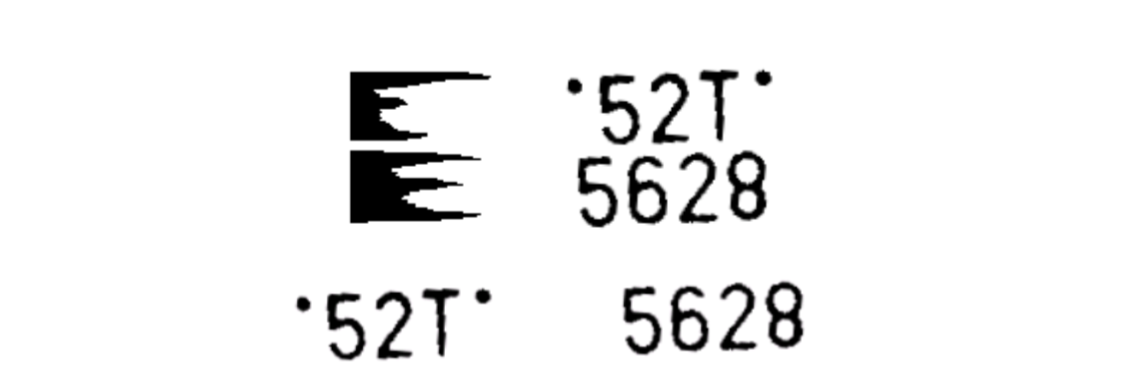
\includegraphics[width=\linewidth]{figures/hough_transformation_1png.png}
  \caption{Rezultatul divizării pe rânduri~\cite{HoughTransformation}}
\end{figure}

\begin{figure}[H]
  \centering
  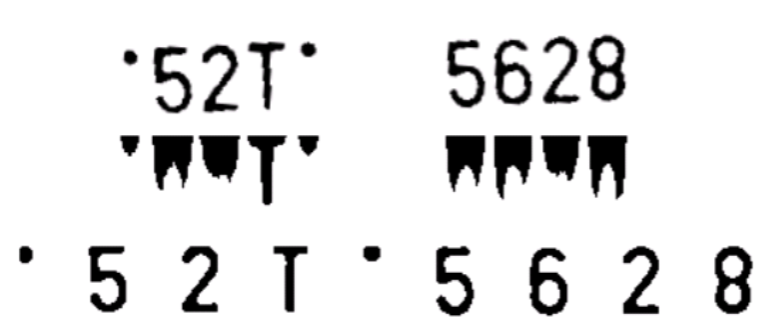
\includegraphics[width=\linewidth]{figures/hough_transformation_2.png}
  \caption{Rezultatul segmentării folosind proiecții verticale~\cite{HoughTransformation}}
  \label{fig:HoughSegmentation}
\end{figure}

\subsection{Utilizarea informațiilor apriori privind aspectul caracterelor}
Cunoștințe apriori în legătură cu aspectul caracterelor, font-ul, mărimea și proporțiile lor pot îmbunătăți în mod semnificativ procesul de segmentare.

În~\cite{sanyuan2004car} este propusă o abordare similară cu cea prezentată anterior în~\cite{HoughTransformation} în care numărul de înmatriculare este adus la o mărime și înclinare standard, iar etapa de segmentare este realizată folosind proiecții orizontale și verticale. Spre deosebire de metoda amintită în mod anterior, autorii se folosesc pe parcursul etapei de segmentare de o structură decizională care va ajuta la eliminarea rezultatelor fals-pozitive.

Particularitatea acestei abordări constă în combinarea informației furnizate de proiecția verticală cu cea obținută printr-o etapă preliminară de analiză a componentelor conexe (pre-extragerea zonelor conexe). Rolul acestei etape preliminare este de a atenua efectul zgomotului asupra proiecției: în prezența zgomotului, profilul de proiecție al imaginii binarizate prezintă punți (conexiuni) între caractere, care îngreunează separarea lor. Prin filtrarea prealabilă a zonelor conexe, numărul acestor conexiuni din profilul de proiecție se reduce semnificativ, motiv pentru care varianta astfel curățată este reținută pentru pașii următori, în detrimentul proiecției obținute direct din imaginea zgomotoasă.

Pe lângă atenuarea zgomotului, zonele conexe pre-extrase furnizează și informațiile apriori care stau la baza extragerii: lățimea caracterelor și poziția lor în cadrul plăcuței. Conform specificului plăcuțelor de înmatriculare avute în vedere, toate caracterele au aceeași lățime, care poate fi estimată direct din lățimea unei zone conexe deja izolate corect (de exemplu cifrele \textit{5} sau \textit{0}). Se definește poziția centrală a unui caracter ca fiind poziția orizontală a marginii sale stângi la care se adaugă jumătate din lățimea caracterului, iar distanța dintre pozițiile centrale a două caractere vecine se numește distanță între pozițiile centrale.

Geometria plăcuței impune o constrângere apriori suplimentară asupra acestor distanțe: ultimele cinci caractere au aceeași distanță între pozițiile centrale, în timp ce distanța $d_0$ dintre al doilea și al treilea caracter este mai mare decât distanța $d_1$ dintre celelalte caractere ($d_0 > d_1$). Experimental, cele două mărimi se află în relația
\begin{equation}
        d_0 = \lambda \cdot d_1, \qquad \lambda \in [1.2,\ 1.3].
\end{equation}

Folosind aceste cunoștințe apriori, procesul de extragere a caracterelor parcurge următorii pași:
\begin{enumerate}
        \item Din zona conexă pre-extrasă se determină intervalul vertical $h_0$ în care se află caracterele plăcuței.
        \item Tot din zona conexă pre-extrasă se obțin lățimea caracterului $w_1$ și pozițiile centrale ale caracterelor, ținând cont de constrângerile geometrice de mai sus (lățime constantă și distanțele $d_0$, $d_1$ dintre pozițiile centrale).
        \item Se scanează zonele conexe cuprinse în intervalul $h_0$ din imaginea plăcuței, integrând informația de poziție furnizată de proiecție; în funcție de rezultat se realizează fie combinarea mai multor zone într-un singur caracter, fie divizarea unei zone care înglobează mai multe caractere.
        \item Se furnizează rezultatul extragerii, care conține pozițiile caracterelor, acestea putând fi astfel izolate cu precizie.
\end{enumerate}

Acest proces adițional de selecție a regiunilor candidat sporește întreaga fiabilitate a sistemului deoarece elementele plăcuței care nu aparțin în-sine de numărul de înmatriculare precum șuruburile de fixare extrase în fig.~\ref{fig:HoughSegmentation} nu vor fi considerate mai departe drept zone de interes.

\subsection{Analiza conturului caracterelor}
O altă abordare are la bază detecția contururilor caracterelor. Pentru aceasta, în~\cite{capar2006concurrent} este propus un proces compus din doi pași, fundamentat pe tehnici de segmentare ce utilizează metoda \textit{Fast Marching} ghidată de formă (shape-driven).

Metoda \textit{Fast Marching}, introdusă de Sethian~\cite{sethian1996fastmarching}, este un algoritm numeric folosit pentru a urmări evoluția unui front (a unei curbe) care se propagă monoton într-o singură direcție, dinspre o regiune inițială către exterior. Algoritmul este o particularizare a metodelor de tip \textit{level-set}, în care viteza de propagare este strict pozitivă, astfel încât odată ce frontul a depășit un punct nu se mai poate întoarce.

Din punct de vedere matematic, metoda calculează, pentru fiecare punct $x$ al imaginii, momentul de timp $T(x)$ la care frontul ajunge în acel punct. Această mărime este soluția ecuației eikonale:
\begin{equation}
        \lvert \nabla T(x) \rvert \, F(x) = 1,
\end{equation}
unde $F(x)$ reprezintă funcția de viteză, care determină cât de rapid avansează frontul în fiecare punct. În aplicațiile de segmentare, funcția de viteză este derivată din informația din imagine (de regulă din magnitudinea gradientului): frontul se deplasează rapid în zonele omogene și încetinește, oprindu-se, în apropierea muchiilor, unde gradientul este mare. În acest fel, contururile obiectelor sunt delimitate în mod natural de zonele în care frontul stagnează.

Particularitatea abordării din~\cite{capar2006concurrent} constă în ghidarea propagării frontului nu doar de informația de contur, ci și de modele statistice ale formei caracterelor (\textit{shape-driven}). Funcția de viteză este astfel construită încât să integreze cunoștințe apriori despre forma caracterelor, permițând curbei să se oprească în dreptul muchiilor reale ale obiectelor și, în același timp, să inspecteze gradul de similaritate dintre conturul obținut și formele caracterelor cunoscute. Procesul realizează concomitent segmentarea și recunoașterea: pe parcursul evoluției frontului sunt determinate atât pozițiile delimitatoare ale fiecărui caracter, cât și eticheta (clasa) caracterului corespunzător, eliminând necesitatea unei etape separate de recunoaștere.
